% !TeX encoding = UTF-8
\documentclass{vip-theme}

% 中文支持
\usepackage{xeCJK}
%\usepackage[UTF8]{ctex}
\linespread{1.47}

% 全文字体
\setmainfont{Times New Roman}

\title{PMBANet: Progressive Multi-Branch Aggregation Network for Scene Depth Super-Resolution}
\author{
	Xinchen Ye , Baoli Sun, Zhihui Wang, Jingyu Yang, Rui Xu , Haojie Li, and Baopu Li %\\[0.5em]
%	$^{1}$School in China \\[0.5em]
%	$^{2}$School in UK
}

\begin{document}


\maketitle
\label{title}

\vspace{0.5em}
\subsection*{Abstract} 
\label{abstract}
Depth map super-resolution is an ill-posed inverse problem with many challenges. First, depth boundaries are generally hard to reconstruct particularly at large magnification factors. Second, depth regions on fine structures and tiny objects in the scene are destroyed seriously by downsampling degradation. To tackle these difficulties, we propose a progressive multi-branch aggregation network (PMBANet), which consists of stacked MBA blocks to fully address the above problems and progressively recover the degraded depth map. Specifically, each MBA block has multiple parallel branches: 1) The reconstruction branch is proposed based on the designed attention-based error feed-forward/-back modules, which iteratively exploits and compensates the downsampling errors to refine the depth map by imposing the attention mechanism on the module to gradually highlight the informative features at depth boundaries. 2) We formulate a separate guidance branch as prior knowledge to help to recover the depth details, in which the multi-scale branch is to learn a multi-scale representation that pays close attention at objects of different scales, while the color branch regularizes the depth map by using auxiliary color information. Then, a fusion block is introduced to adaptively fuse and select the discriminative features from all the branches. The design methodology of our whole network is well-founded, and extensive experiments on benchmark datasets demonstrate that our method achieves superior performance in comparison with the state-of-the-art methods. Our code and models are available at \href{https://github.com/Sunbaoli/PMBANet\_DSR/}{https://github.com/Sunbaoli/PMBANet\_DSR/}.


\section{Motivation}
\label{motivation}

深度图像超分辨率重建是一个病态的逆问题。由于低分辨率深度图像包含的信息有限,深度场景的边缘和细节作为高频信息通常很难精确地从有限的低分辨率深度信息中恢复,尤其在上采样倍率较大的情况下,容易造成重建的高分辨率深度图像损失清晰度。其次,深度场景的精细结构和微小目标在降采样过程中受到的破坏更加严重,进一步阻碍了深度图像的精确恢复。

\begin{figure}[!htbp]
\centering
	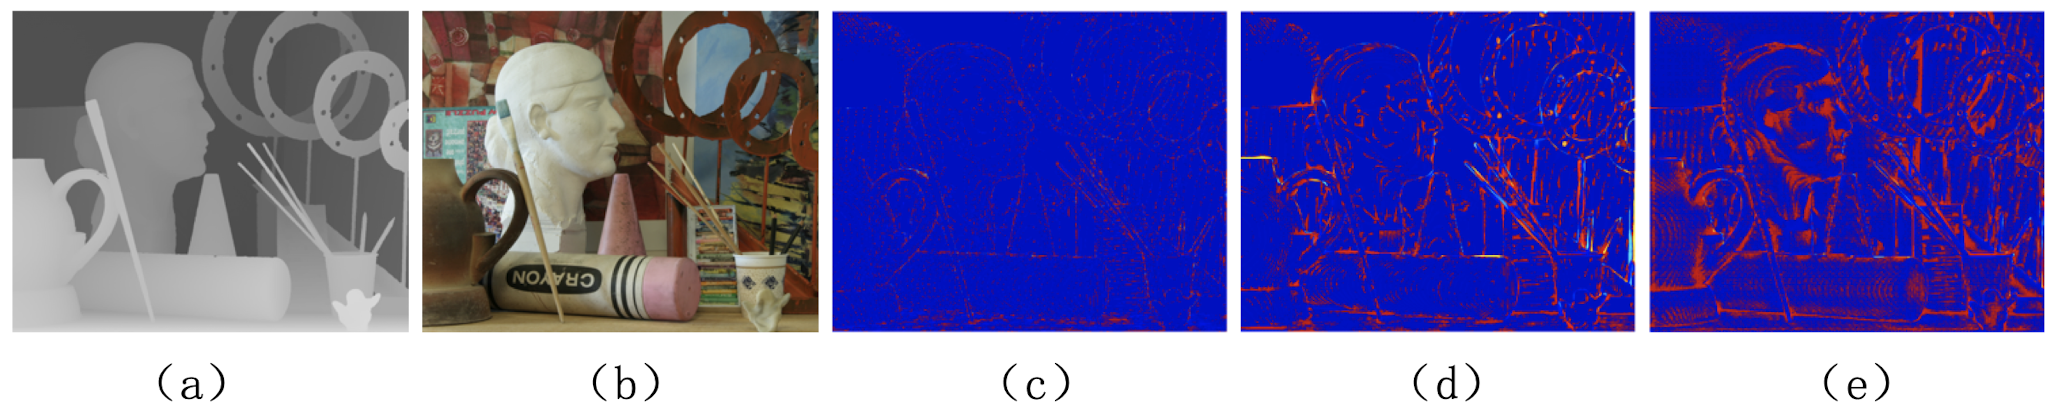
\includegraphics[width=\textwidth]{figure/motivation}
	\caption{(a)深度图像 ground truth;(b)彩色图像;重建深度图像与深度图像 ground truth 的误差图:(c)$4\times$;(d)$8\times$;(e)$16\times$ }
	\label{fig:motivation}
\end{figure}

如图 \ref{fig:motivation}(c)-(e)所示,重建的深度图像与真实深度图像的误差较大的区域大多出现在深度图像的结构边缘和微小物体区域,例如图中的木棍和圆圈边缘,而这些也正是深度图像超分辨率要去解决的问题。

此外,在颜色指导的深度图像超分辨率重建方法中,彩色图像与深度图像的结构并不总是一致的,可能会导致明显的伪像,例如纹理复制和深度泄漏。因此,如何利用颜色信息来帮助恢复深度图像以及是否所有的上采样倍率(特别是对于容易恢复的 $2\times$ 和 $4\times$ 上采样倍率)都需要彩色图像的指导,还有待探讨和验证。


\section{Contribution}
\label{contribution}

本文的主要贡献可总结如下:
\begin{enumerate}
	
	\item[(1)]	提出的并行的网络架构继承了集成学习(ensemble learning)的优势,可以从每个分支学习有益的和多样化的特征。融合块在渐进网络中通过自适应地为多分支的特征分配权重来进行信息融合;
\item[(2)]	基于前馈/反馈连接和注意力机制设计了一种新颖的骨干网络(RB),以增强高分辨率表示;
\item[(3)]	通过密集连接和空洞卷积的重组构造独立的多尺度分支(MB),以更好地捕获多尺度信息;
\item[(4)]	消融实验中验证了颜色信息仅适合在较早的阶段引入以帮助深度图像的重建,在上采样倍率为 $8\times$/$16\times$ 的情况下,可以提供明显的帮助并显著改善任务性能,但对容易恢复的上采样倍率为 $2\times$/$4\times$ 的情况却没有帮助更甚至有反向作用。
\end{enumerate}


\section{Method}
\label{method}


传统来讲,颜色引导的深度图像超分辨率重建方法被公示话为一个优化问题,这一优化问题通过一个保真项(fidelity term)和一个先验项来对超分辨率重建的病态问题进行约束,大体上将其归约为以下优化函数:

\begin{equation}
x^{*}=\underset{x}{\arg \min } \frac{1}{2}\|y-K x\|^{2}+\lambda \sum_{l} \omega_{l} * \rho_{l}\left(f_{l} \otimes x\right)
\end{equation}

其中,$K$ 是下采样退化矩阵, $\lambda$ 为平衡(trade-off)参数。 $f_l$ 和 $\rho_l(·)$ 为一组滤波器核函数和惩罚函数$^1$。\marginpar[1]{\footnotesize $^1$filtering kernels and penalty functions} $\omega$ 是由相应的彩色图像计算得到的加权矩阵。 $\otimes$ 为卷积操作。

这些方法的关键是对先验项部分的设计,但这些人为提取的特征并不能接近真实的图像先验。在一些基于模型的优化方法中采用了即插即用的降噪器,并根据给定的算法推导出特定的迭代方案来计算出最优的“答案”。

然而,$K$ 中的未知因素$^2$\marginpar[1]{\footnotesize $^2$例如,包括一些混合退化(噪声、深度缺失和下采样)}导致难以用有限的表示建模保真项。此外,现有的 CNN 降噪器不是专门为深度超分辨率重建任务设计的,导致深度超分中使用的颜色信息和多尺度信息经常被忽略。

基于上述分析,本文旨在追求更好的深度图像超分辨率重建任务的模型架构设计,进而提升深度图像超分辨率重建任务的性能。

本文提出的渐进式多路聚合的深度图像超分辨率网络(progressive multi-branch aggregation network, PMBANet),由堆叠的多分路聚合块(multi branch aggregation, MBA)组成,以逐步恢复退化的深度图像。

\begin{figure*}[!htbp]
\centering
	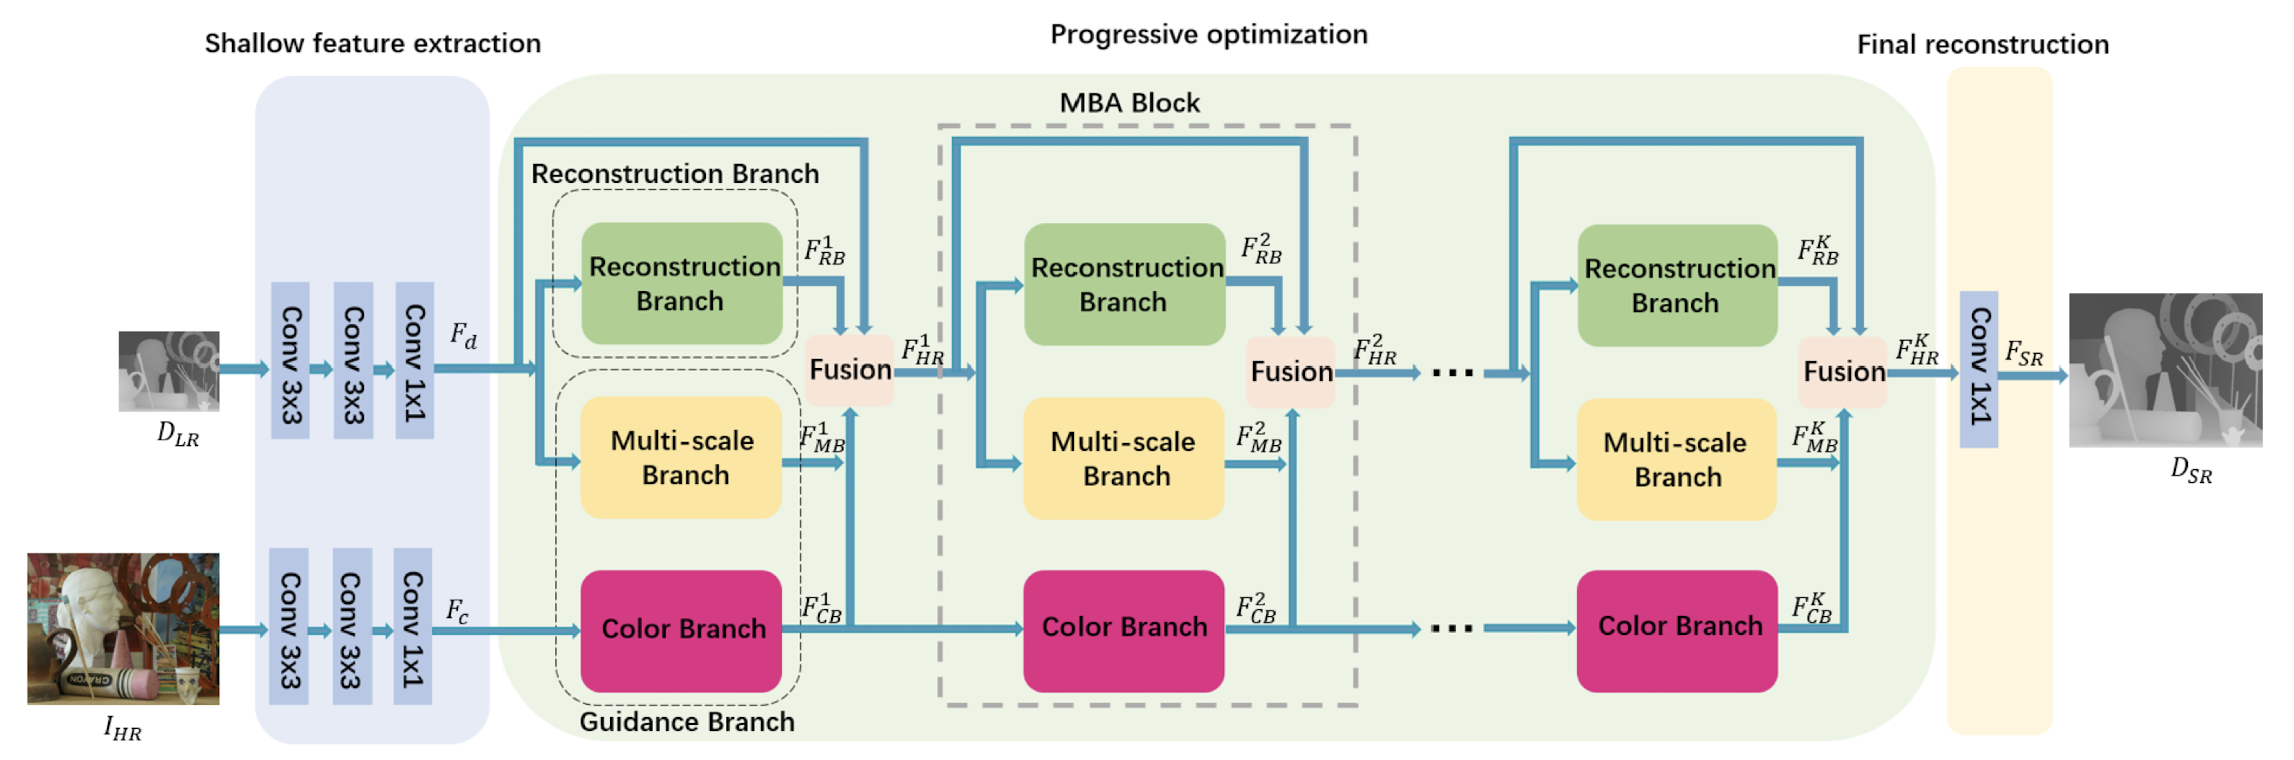
\includegraphics[width=.7\paperwidth]{figure/model.png}
	\caption{PMBANet 的网络架构。为了更好地呈现整个框架和实现细节,使用不同颜色的矩形来表示不同的阶段和每个阶段的不同操作。}
	\label{fig:model}
\end{figure*}

首先对渐进式多路聚合的深度图像超分辨率网络的整体结构进行介绍,如图 \ref{fig:model} 所示。该网络包含三个阶段:

\begin{enumerate}
	\item[(1)] \textbf{浅层特征提取阶段(Shallow feature extraction)}
	在进入渐进优化阶段之前,首先通过浅层卷积层分别从低分辨率的深度图($D_{LR}$)和高分辨率的彩色图($I_{HR}$)提取初始深度特征 $F_d$ 和颜色特征 $F_c$ 。$F_d$ 下一阶段作为输入被送入到重建支路和指导支路,而 $F_c$ 仅被送入到指导支路。
	\item[(2)] \textbf{渐进优化阶段(Progressive optimization)} 优化阶段由 K 个堆叠的 MBA 块组成。每个 MBA 块有两个并行的支路,即重建支路(Reconstruction Branch,RB)和指导支路(Guidance Branch,GB)。然后,利用融合块自适应融合 RB 和 GB 的特征,并且从两个分支中选择判别性的特征。通过堆叠的 MBA 块,丢失的深度细节在高分辨率特征空间逐步恢复。
	\begin{enumerate}
		\item[1)] \textbf{重建支路(Reconstruciton Branch, RB)} 基于注意力的错误前馈/反馈模块(attention-based error feed-forward/back modules, AF)而设计,通过在前馈/反馈过程中引入注意机制使得网络在低分辨率特征空间和高分辨率特征空间上获取深度图像的结构等高频信息;

		\item[2)] \textbf{指导支路(Guidance Branch, GB)} 包括一个多尺度特征学习模块(Multi-scale Branch, MB)和一个彩色特征提取模块(Color Branch,CB),该支路为一个独立的子网以帮助 RB 恢复深度细节;
		\begin{itemize}
			\item MB 学习的是多尺度表示,密切关注不同尺度的对象;
			\item CB 则基于深度-颜色图像对之间的结构相似性,通过颜色信息的辅助来深度图像进行正则化。
		\end{itemize}

	\item[3)] \textbf{融合块(Fusion Block, FB)} 基于通道注意力机制在通道层面融合重建支路和指导支路的特征,进一步选择并且挖掘有效的信息提升深度图像重建的性能。

 
	\end{enumerate}
	\item[(3)] \textbf{最后重建阶段(Final reconstruction)} 在最后一个 MBA 块的输出特征图使用 $1\times 1$ 卷积将特征映射到深度图像空间,得到重建的超分辨深度图像。
\end{enumerate}

\subsection{重建支路}

\begin{figure}[!htbp]
	\begin{minipage}[t]{0.5\linewidth}
		\centering
		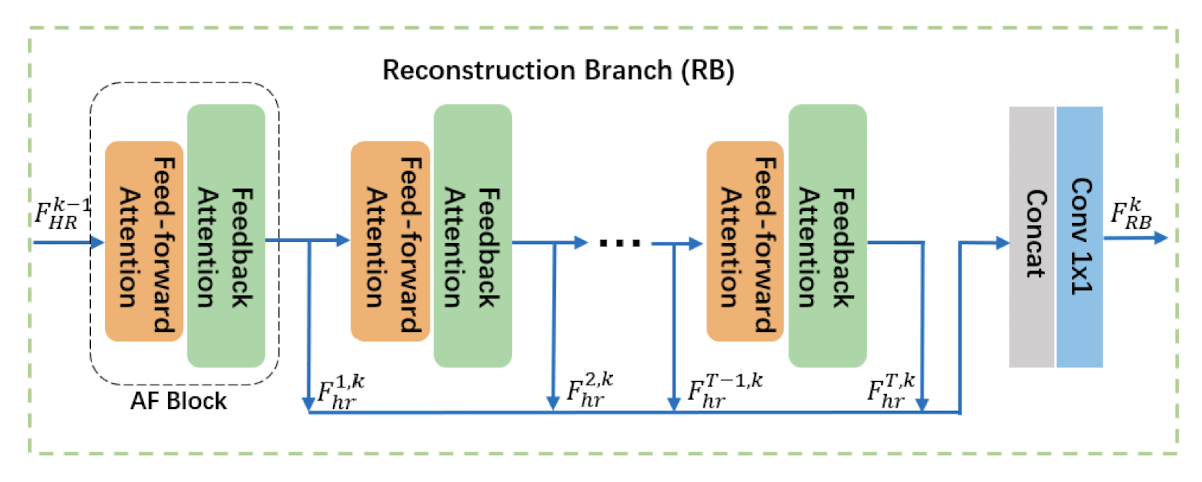
\includegraphics[height=1.5in,width=2.8in]{figure/RB}
		\caption{重建支路}
		\label{fig:RB}
	\end{minipage}
	\begin{minipage}[t]{0.5\linewidth}
		\centering
		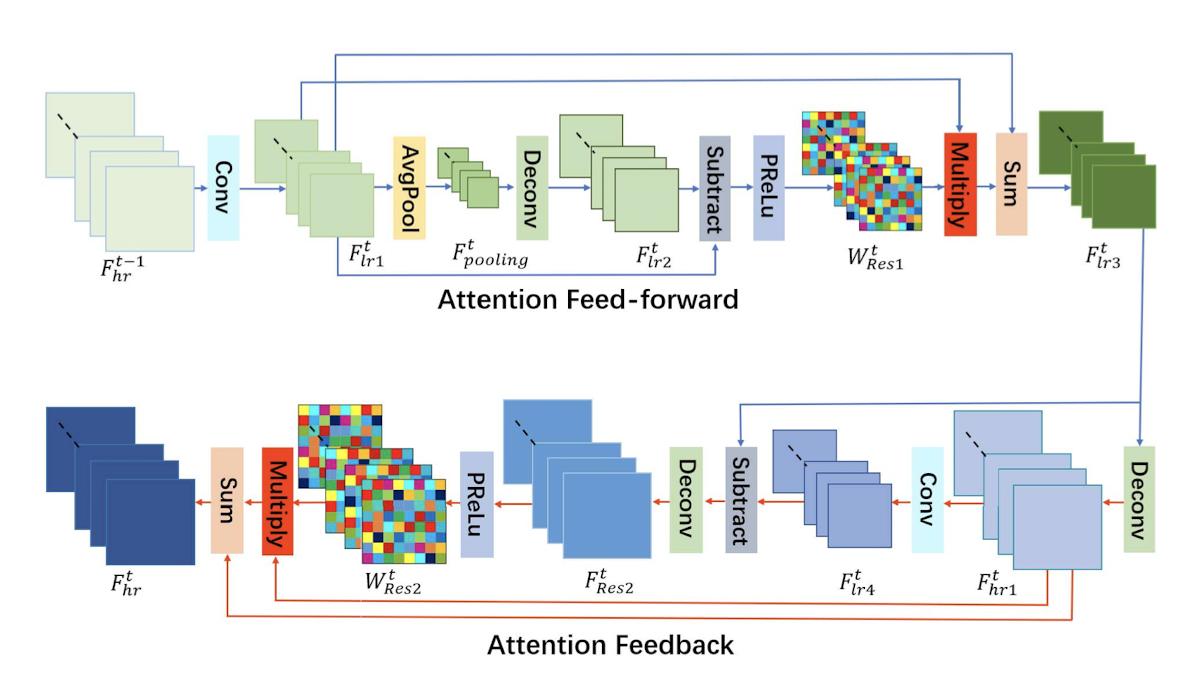
\includegraphics[height=1.5in,width=2.8in]{figure/AF}
		\caption{基于注意力的误差反馈模块 }
		\label{fig:AF}
	\end{minipage}
\end{figure}

深度图像是由一些表示场景结构的深度边界及其分隔的光滑区域组成,真正影响深度图像重建质量的是边界的重建精度。受反馈机制$^3$\marginpar{\footnotesize $^3$反馈机制,也就是传统算法中的反向投影,已经被应用到各种计算机视觉任务中。首先,针对图像配准问题提出了基于反馈机制的反投影算法,该算法在亚像素精度的基础上迭代提高图像分辨率。}和自注意力机制$^4$\marginpar{\footnotesize $^4$自注意机制被广泛用于对特征的内部表示进行建模,并通过关注一组特征映射来选择更有信息的特征,捕获特征的相互依赖性。}的启发,本文的网络设计使用反馈连接来有效地捕捉深度边界附近的高频特征,然后利用空间注意机制自动突出和增强提取的高频特征。结合上述两种技术,提出了一种以深度细节恢复能力为重点的网络模型,即基于注意力的误差反馈模块(Attention Feedforward/-back,AF)\footnote{现有的深度图像超分辨率重建网络大多使用的是后上采样模式或者渐进上采样模式,但这些模式仅关注到了低分辨率到高分辨率的信息传播,忽略了高分辨率到低分辨率的传播,即忽略了高分辨率与低分辨率特征的相互映射关系。本文提出的模型则是基于低分辨率深度图像与高分辨率深度图像的依赖关系。},如图 \ref{fig:AF} 所示。

基于注意力的误差反馈模块包括两个阶段:基于注意力的前馈阶段(强调低分辨率域的特征)和基于注意力的反馈阶段(进一步加强高分辨率域的有效特征)。第 $i$ 个 AF 块的基于注意力的前馈阶段定义如下:


\begin{equation}
\begin{aligned}
F_{l r 1}^{t} &=\text { Down }^{t}\left(F_{h r}^{t-1}\right)\\
F_{\text {pooling }}^{t} &=\operatorname{Avgpool}^{t}\left(F_{l r 1}^{t}, j\right)\\
F_{l r 2}^{t} &=U p^{t}\left(F_{\text {pooling }}^{t}\right)\\
W_{\text {Res1 }}^{t} &=P \operatorname{Rel} u^{t}\left(F_{l r 2}^{t}-F_{l r 1}^{t}\right)\\
F_{l r 3}^{t} &=F_{l r 1}^{t}+\gamma\left(F_{l r 1}^{t} * W_{\text {Res } 1}^{t}\right)
\end{aligned}
\end{equation}

\textbf{前馈阶段}的输入为上一个基于注意力的误差反馈模块的输出 $F_{h r}^{t-1}$($t=1$ 时,基于注意力的误差反馈模块的输入为浅层特征提取阶段的输出 $F_d$),首先通过一个卷积层将输入下采样到 LR 空间得到特征图 $F_{l r 1}^{t}$;然后经过一个平均池化层进一步压缩 $F_{l r 1}^{t}$ 的分辨率得到特征图 $F_{\text {pooling }}^{t} $,其中 $j$ 为池化操作的下采样倍率。将压缩后的特征 $F_{\text {pooling }}^{t} $ 再在经过反卷积操作上采样回原分辨率空间得到 $F_{l r 2}^{t}$,$F_{l r 2}^{t}$ 与压缩之前的特征 $F_{l r 1}^{t}$ 的空间分辨率相同;通过激活 $F_{l r 2}^{t}$ 与 $F_{l r 1}^{t}$ 的残差,得到 LR 空间的特征图的注意力图,这个注意力图用来强调深度图像在 LR 空间的高频区域。

将注意力图 $W_{\text {Res1 }}^{t}$ 与 $F_{l r 1}^{t}$ 进行对应元素相乘,使得网络关注到 $F_{l r 1}^{t}$ 中的高频区域,提升对深度图像中高频组件(结构边缘)的恢复。$\gamma$ 是一个平衡参数。

\textbf{反馈阶段}的操作与前馈阶段相似,不同点在于反馈阶段是对 HR 空间的特征上进行操作。首先将前馈阶段的输出 $F_{l r 3}^{t}$ 上采样到 HR 空间得到特征图 $F_{h r 1}^{t}$,然后经过一个卷积层将 $F_{h r 1}^{t}$ 下采样到 LR 空间得到特征$F_{l r 4}^{t}$;将 $F_{l r 4}^{t}$ 与 $F_{l r 3}^{t}$ 的残差上采样到 HR 空间,通过激活这个特征残差得到 HR 空间的注意力图,这个注意力图用来强调深度图像在 HR 空间的高频区域。

将注意力图 $W_{R e s 2}^{t}$ 与 $F_{h r 1}^{t}	$ 进行对应元素相乘,得到反馈阶段的输出 $F_{h r}^{t}$。

\begin{equation}
\begin{aligned}
F_{h r 1}^{t} &=U p^{t}\left(F_{l r 3}^{t}\right) \\
F_{l r 4}^{t} &=\operatorname{Down}^{t}\left(F_{h r 1}^{t}\right) \\
F_{R e s 2}^{t} &=U p^{t}\left(F_{l r 4}^{t}-F_{l r 3}^{t}\right) \\
W_{R e s 2}^{t} &=P \operatorname{Rel} u^{t}\left(F_{R e s 2}^{t}\right) \\
F_{h r}^{t} &=F_{h r 1}^{t}+\gamma\left(F_{h r 1}^{t} * W_{R e s 2}^{t}\right)
\end{aligned}
\end{equation}

如图 \ref{fig:RB} 所示,重建支路由 T 个基于注意力的误差反馈模块构成,再将每个模块的高分辨率特征 $F_{h r}^{t}$ 串联在一起,最后由一个简单的卷积层进行初步融合,这样就得到了第 $k$ 个多路聚合模块的输出深度特征 $F_{R B}^{k}$。

\begin{equation}
F_{R B}^{k}=\operatorname{Conv}_{1 \times 1}^{k}\left(\left[F_{h r}^{1, k}, F_{h r}^{2, k}, \ldots, F_{h r}^{T, k}\right]\right)
\end{equation}

其中,$\operatorname{Conv}_{1 \times 1}$ 表示卷积核大小为 $1 \times 1$ 的卷积层,$[\cdot]$ 为级联操作。

\subsection{指导支路}

\begin{figure}[!htbp]
	\begin{minipage}[t]{0.5\linewidth}
		\centering
		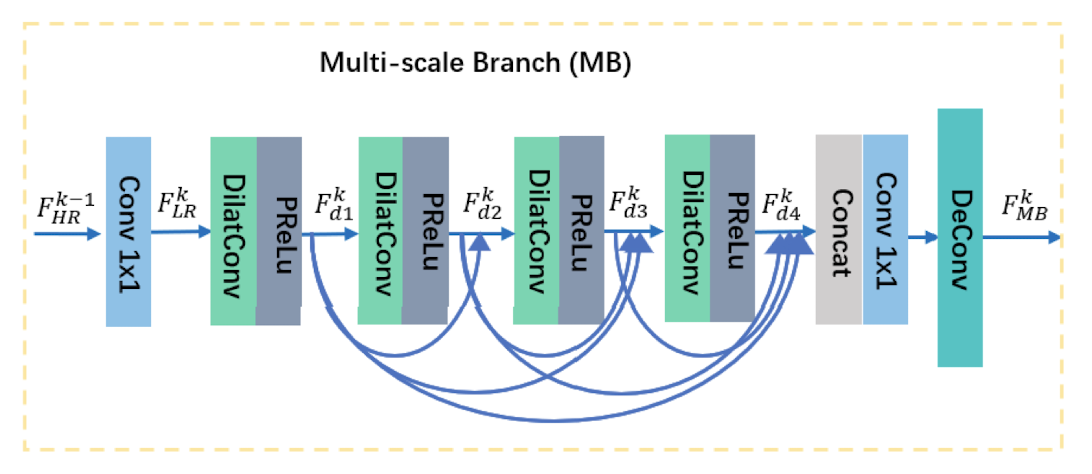
\includegraphics[height=1.5in,width=2.8in]{figure/MB}
		\caption{多尺度支路}
		\label{fig:MB}
	\end{minipage}
	\begin{minipage}[t]{0.5\linewidth}
		\centering
		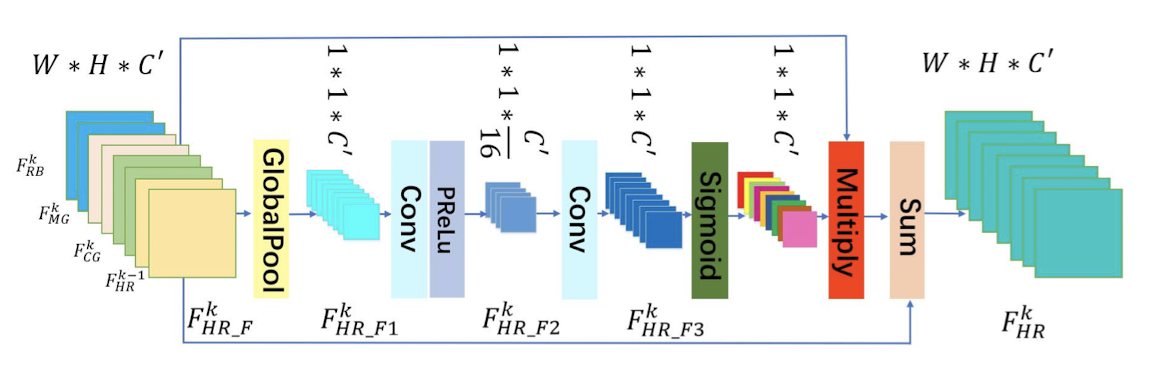
\includegraphics[height=1.2in,width=2.8in]{figure/FB}
		\caption{融合模块}
		\label{fig:FB}
	\end{minipage}
\end{figure}



\subsubsection{多尺度特征学习支路}

有效的多尺度信息对于解决下采样对多尺度对象的影响不同的问题至关重要。多尺度特征学习支路利\footnote{与之前将多尺度技术结合到骨干网络中的方法不同,本文的网络设计从骨干网络中构造一个独立的支路来建模多尺度问题,从而更有效地提取多尺度特征表示。}用四个空洞卷积及紧随其后的 PReLu,在不改变输入特征分辨率的前提下获取多尺度的深度感受野。此外,多尺度特征学习支路利用稠密连接的方式,在缓解梯度消失的同时,使得每一特定层扩张卷积都可以处理不同阶段的所有特征,从而获取更加精细的多尺度信息,每一层的空洞卷积输出特征 $F_{d_{i}}^{k}$。

\begin{equation}
F_{d_{i}}^{k}=\operatorname{DilatConv}\left(\left[F_{d_{1}}^{k}, \ldots, F_{d_{i-1}}^{k}\right], i\right), \quad i=2,3,4
\end{equation}

式中,$\operatorname{DilatConv}(\cdot)$ 表示空洞卷积层,$i$ 表示第 $i$ 个空洞卷积层,$d_i$ 表示空洞率。最后串连每层扩张卷积的输出,通过一个卷积核大小为 $1\times 1$ 的卷积层减少特征通道,再通过一个反卷积层将多尺度特征上采样到目标尺寸,得到多尺度特征支路的输出 $F_{M B}^{k}$。
\begin{equation}
F_{M B}^{k}=\operatorname{DeConv}\left(\operatorname{Conv}_{1 \times 1}\left(\left[F_{d_{1}}^{k}, F_{d_{2}}^{k}, F_{d_{3}}^{k}, F_{d_{4}}^{k}\right]\right)\right)
\end{equation}

\subsubsection{彩色特征提取支路}

高分辨率彩色图像可以显著提升深度图像超分辨率重建任务的性能,但由于彩色图像和深度图像的纹理存在较大差异,可能会导致纹理复制的问题。本文的网络使用彩色图像作为补充信息,将彩色特征与深度特征进行了融合。在后续的实验中,也验证了将彩色信息整合到网络中的合适位置,以及不同下采样情况下使用彩色信息作为指导的适用性,这些都是现有方法没有关注到的方向。彩色指导支路使用 3 层连续的卷积层,卷积核的尺寸分别为 $3\times 3$,$3\times 3$ 和 $1\times 1$,得到彩色指导特征 $F_{CB}^k$。



\subsection{融合模块}
融合模块(Fusion Block)的目标是有效地挖掘不同支路的特征不同通道之间的关系,选择有用的通道进一步提升深度图像超分辨率重建任务的性能。通道注意力$^5$\marginpar{\footnotesize $^5$通道注意力机制目的在于学习图像特征在通道维度的权重分布,然后应用学习到的权重到原始特征,使得对应任务聚焦到关键特征通道忽略一些次要特征。}非常适合融合模块去自适性地聚合不同支路的特征。定义融合模块来融合第 $k$ 个多路聚合块的输出特征 $F_{RB}^k$,$F_{MB}^k$,$F_{CB}^k$ 以及第 $k-1$ 个多路聚合块的融合后的特征 $F_{HR}^{k-1}$,如图 \ref{fig:FB} 所示,融合模块的具体做法如下:

\begin{equation}
\begin{aligned}
F_{H R_{-} F}^{k} &=\left[F_{R B}^{k}, F_{M B}^{k}, F_{C B}^{k}, F_{H R}^{k-1}\right] \\
F_{H R_{-} F 1}^{k} &=\text { Globalpool }^{k}\left(F_{H R_{-} F}^{k}\right) \\
F_{H R_{-} F 2}^{k} &=\text { Conv } v_{1}^{k}\left(F_{H R_{-} F 1}^{k}\right) \\
F_{H R_{-} F 3}^{k} &=\text { Conv } v_{2}^{k}\left(F_{H R_{-} F 2}^{k}\right) \\
F_{H R}^{k} &=F_{H R_{-} F}^{k}+F_{H R_{-} F}^{k} * \sigma\left(F_{H R_{-} F 3}^{k}\right)
\end{aligned}
\end{equation}

其中,$[\cdot]$ 表示级联操作,$\text { Globalpool }^{k}$ 表示全局平均池化层用来将串联后的特征 $F_{HR\_F}^k$ 压缩为一个特征向量 $F_{HR\_F1}^k$。然后,使用两个卷积层进一步学习 $F_{HR\_F}^k$ 中各个通道之间的统计相关性。$\sigma$ 是一个 Sigmoid 激活操作。最终得到经过重新赋予权重的融合特征 $F_{HR}^k$。


综上所述,\textbf{本文设计了两个并行分支 RB 和 GB,分别对保真项和先验项进行建模,同时引入了一个融合模块来对两个支路进行聚合,而不是使用参数 $\lambda$ 的简单求和}。通过迭代优化和聚合,逐步恢复退化的深度图像。基于反馈机制和自注意力机制设计的 RB 可以更好地利用 HR 特征。与其对保真项项进行硬编码,本文让网络自由学习 $K$ 。对于 GB,为了更好地表征滤波器组 $f_l$,本文设计了一个基于不同空洞率的多尺度支路,且起通过密集连接来提取不同视野的各种特征。每个空洞后使用 PReLu 作为非线性惩罚。此外,颜色支路也用作先验知识以进一步利用颜色特征帮助恢复退化的深度图。 GB 与 RB 一起动态调整以进行优化。整个网络的设计方法源于基于模型的优化方法,但同时使用深度网络对保真项和先验项进行建模。

\section{Experiments}
\label{experimentes}

以 MIDDLEBURY 数据集为例,首先在四个常见倍率($2\times$、$4\times$、$8\times$ 和 $16\times$)的超分辨率任务上对比了多个先进的算法,如表 \ref{tab:middlebury} 所示。传统的基于过滤或优化的方法比基于深度学习的方法获得了更高的 MAD 值(MAD 越低代表性能更好),在这些基于深度学习的方法中,PMBANet 几乎获得了最好的客观结果,特别是对于较难恢复的上采样倍率为 $8\times$ 和 $16\times$ 的情况。

\begin{table*}[!htbp]
\tiny
\caption{在 Middlebury 2005 数据集上的性能对比}
\label{tab:middlebury}
\renewcommand{\arraystretch}{1.2}
		\setlength{\tabcolsep}{.25mm}{
\begin{tabular}{c|ccc|ccc|ccc|ccc|ccc|ccc}
\hline
\multirow{2}{*}{} & \multicolumn{3}{c|}{Art} & \multicolumn{3}{c|}{Books} & \multicolumn{3}{c|}{Dolls} & \multicolumn{3}{c|}{Laundry} & \multicolumn{3}{c|}{Mobius} & \multicolumn{3}{c}{Reindeer} \\
\cline{2-19}
 &$\times 4$  &$\times 8$  &  $\times 16$& $\times 4$ & $\times 8$ & $\times 16$ & $\times 4$ & $\times 8$ & $\times 16$ & $\times 4$ & $\times 8$ & $\times 16$ & $\times 4$ & $\times 8$ & $\times 16$ & $\times 4$ & $\times 8$ & $\times 16$ \\
 \hline
CLMF & 0.76/{\color{blue}8.12} & 1.44/{\color{blue}17.28} & 2.87/{\color{blue}33.25} & 0.28/{\color{blue}3.27} & 0.51/{\color{blue}7.25} & 1.02/{\color{blue}16.09} & 0.34/{\color{blue}4.40} & 0.60/{\color{blue}8.76 } & 1.01/{\color{blue}18.32} & 0.50/{\color{blue}5.50} & 0.80/{\color{blue}12.67} & 1.67/{\color{blue}25.40} & 0.29/{\color{blue}4.13} & 0.51/{\color{blue}8.42} & 0.97/{\color{blue}17.27} & 0.51/{\color{blue}4.65} & 0.84/{\color{blue}9.96 } & 1.55/{\color{blue}18.34} \\
JGF  & 0.47/{\color{blue}3.25} & 0.78/{\color{blue}7.39 } & 1.54/{\color{blue}14.31} & 0.24/{\color{blue}2.14} & 0.43/{\color{blue}5.41} & 0.81/{\color{blue}12.05} & 0.33/{\color{blue}3.23} & 0.59/{\color{blue}7.29 } & 1.06/{\color{blue}15.87} & 0.36/{\color{blue}2.60} & 0.64/{\color{blue}4.54 } & 1.20/{\color{blue}8.69 } & 0.25/{\color{blue}3.36} & 0.46/{\color{blue}6.45} & 0.80/{\color{blue}12.33} & 0.38/{\color{blue}2.27} & 0.64/{\color{blue}5.17 } & 1.09/{\color{blue}11.84} \\
EDGE & 0.65/{\color{blue}6.82} & 1.03/{\color{blue}13.49} & 2.11/{\color{blue}25.90} & 0.30/{\color{blue}3.35} & 0.56/{\color{blue}8.50} & 1.03/{\color{blue}19.32} & 0.31/{\color{blue}2.90} & 0.56/{\color{blue}6.84 } & 1.05/{\color{blue}17.97} & 0.32/{\color{blue}2.82} & 0.54/{\color{blue}5.46 } & 1.14/{\color{blue}13.57} & 0.29/{\color{blue}3.72} & 0.51/{\color{blue}7.36} & 1.10/{\color{blue}14.05} & 0.37/{\color{blue}2.67} & 0.63/{\color{blue}6.22 } & 1.28/{\color{blue}16.80} \\
TGV  & 0.65/{\color{blue}5.14} & 1.17/{\color{blue}10.51} & 2.30/{\color{blue}21.37} & 0.27/{\color{blue}2.48} & 0.42/{\color{blue}4.65} & 0.82/{\color{blue}11.20} & 0.33/{\color{blue}4.45} & 0.70/{\color{blue}11.12} & 2.20/{\color{blue}45.54} & 0.55/{\color{blue}6.99} & 1.22/{\color{blue}16.32} & 3.37/{\color{blue}53.61} & 0.29/{\color{blue}3.68} & 0.49/{\color{blue}6.84} & 0.90/{\color{blue}14.09} & 0.49/{\color{blue}4.67} & 1.03/{\color{blue}11.22} & 3.05/{\color{blue}43.48} \\
KSVD & 0.64/{\color{blue}3.46} & 0.81/{\color{blue}5.18 } & 1.47/{\color{blue}8.39 } & 0.23/{\color{blue}2.13} & 0.52/{\color{blue}3.97} & 0.76/{\color{blue}8.76 } & 0.34/{\color{blue}4.53} & 0.56/{\color{blue}6.18 } & 0.82/{\color{blue}12.98} & 0.35/{\color{blue}2.19} & 0.52/{\color{blue}3.89 } & 1.08/{\color{blue}8.79 } & 0.28/{\color{blue}2.08} & 0.48/{\color{blue}4.86} & 0.81/{\color{blue}8.97 } & 0.47/{\color{blue}2.19} & 0.57/{\color{blue}5.76 } & 0.99/{\color{blue}12.67} \\
CDLLC & 0.53/{\color{blue}2.86} & 0.76/{\color{blue}4.59 } & 1.41/{\color{blue}7.53 } & 0.19/{\color{blue}1.34} & 0.46/{\color{blue}3.67} & 0.75/{\color{blue}8.12 } & 0.31/{\color{blue}4.61} & 0.53/{\color{blue}5.94 } & 0.79/{\color{blue}12.64} & 0.30/{\color{blue}2.08} & 0.48/{\color{blue}3.77 } & 0.96/{\color{blue}8.25 } & 0.27/{\color{blue}1.98} & 0.46/{\color{blue}4.59} & 0.79/{\color{blue}7.89 } & 0.43/{\color{blue}2.09} & 0.55/{\color{blue}5.39 } & 0.98/{\color{blue}11.49} \\
PB  & 0.79/{\color{blue}3.12} & 0.93/{\color{blue}6.18 } & 1.98/{\color{blue}12.34} & 0.16/{\color{blue}1.39} & 0.43/{\color{blue}3.34} & 0.79/{\color{blue}8.12 } & 0.53/{\color{blue}3.99} & 0.83/{\color{blue}6.22 } & 0.99/{\color{blue}12.86} & 1.13/{\color{blue}2.68} & 1.89/{\color{blue}5.62 } & 2.87/{\color{blue}11.76} & 0.17/{\color{blue}1.95} & 0.47/{\color{blue}4.12} & 0.82/{\color{blue}8.32 } & 0.56/{\color{blue}6.04} & 0.97/{\color{blue}12.17} & 1.89/{\color{blue}21.35} \\
EG  & 0.48/{\color{blue}2.48} & 0.71/{\color{blue}\textbf{3.31} } & 1.35/{\color{blue}\textbf{5.88} } & 0.15/{\color{blue}1.23} & 0.36/{\color{blue}3.09} & 0.70/{\color{blue}7.58 } & 0.27/{\color{blue}2.72} & 0.49/{\color{blue}5.59 } & 0.74/{\color{blue}12.06} & 0.28/{\color{blue}1.62} & 0.45/{\color{blue}2.86 } & 0.92/{\color{blue}7.87 } & 0.23/{\color{blue}1.88} & 0.42/{\color{blue}4.29} & 0.75/{\color{blue}7.63 } & 0.36/{\color{blue}1.97} & 0.51/{\color{blue}4.31 } & 0.95/{\color{blue}9.27}  \\
SRCNN & 0.63/{\color{blue}7.61} & 1.21/{\color{blue}14.54} & 2.34/{\color{blue}23.65} & 0.25/{\color{blue}2.88} & 0.52/{\color{blue}7.98} & 0.97/{\color{blue}15.24} & 0.29/{\color{blue}3.93} & 0.58/{\color{blue}8.34 } & 1.03/{\color{blue}16.13} & 0.40/{\color{blue}6.25} & 0.87/{\color{blue}13.63} & 1.74/{\color{blue}24.84} & 0.25/{\color{blue}3.63} & 0.43/{\color{blue}7.28} & 0.87/{\color{blue}14.53} & 0.35/{\color{blue}3.84} & 0.75/{\color{blue}7.98 } & 1.47/{\color{blue}14.78} \\
DSP  & 0.73/{\color{blue}7.83} & 1.56/{\color{blue}15.21} & 3.03/{\color{blue}31.32} & 0.28/{\color{blue}3.19} & 0.61/{\color{blue}8.52} & 1.31/{\color{blue}16.73} & 0.32/{\color{blue}4.74} & 0.65/{\color{blue}9.53 } & 1.45/{\color{blue}19.37} & 0.45/{\color{blue}6.19} & 0.98/{\color{blue}12.86} & 2.01/{\color{blue}22.96} & 0.31/{\color{blue}3.89} & 0.59/{\color{blue}8.23} & 1.26/{\color{blue}16.58} & 0.42/{\color{blue}3.59} & 0.84/{\color{blue}7.23 } & 1.73/{\color{blue}14.12} \\
ATGVNet & 0.65/{\color{blue}3.78} & 0.81/{\color{blue}3.78 } & 1.42/{\color{blue}9.68 } & 0.43/{\color{blue}5.48} & 0.51/{\color{blue}7.16} & 0.79/{\color{blue}10.32} & 0.41/{\color{blue}4.55} & 0.52/{\color{blue}6.27 } & \textbf{0.56}/{\color{blue}12.64} & 0.37/{\color{blue}2.07} & 0.89/{\color{blue}3.78 } & 0.94/{\color{blue}8.69 } & 0.38/{\color{blue}3.47} & 0.45/{\color{blue}4.81} & 0.80/{\color{blue}8.56 } & 0.41/{\color{blue}3.82} & 0.58/{\color{blue}5.68 } & 1.01/{\color{blue}12.63} \\
MSG  & 0.46/{\color{blue}2.31} & 0.76/{\color{blue}4.31 } & 1.53/{\color{blue}8.78 } & 0.15/{\color{blue}1.21} & 0.41/{\color{blue}3.24} & 0.76/{\color{blue}7.85 } & 0.25/{\color{blue}2.39} & 0.51/{\color{blue}4.86 } & 0.87/{\color{blue}9.94 } & 0.30/{\color{blue}1.68} & 0.46/{\color{blue}2.78 } & 1.12/{\color{blue}7.62 } & 0.21/{\color{blue}1.79} & 0.43/{\color{blue}4.05} & 0.76/{\color{blue}7.48 } & 0.31/{\color{blue}1.73} & 0.52/{\color{blue}2.93 } & 0.99/{\color{blue}7.63}  \\
DGDIE  & 0.48/{\color{blue}2.34} & 1.20/{\color{blue}13.18} & 2.44/{\color{blue}26.32} & 0.30/{\color{blue}3.21} & 0.58/{\color{blue}7.33} & 1.02/{\color{blue}14.25} & 0.34/{\color{blue}4.79} & 0.63/{\color{blue}9.44 } & 0.93/{\color{blue}11.66} & 0.35/{\color{blue}2.03} & 0.86/{\color{blue}3.69 } & 1.56/{\color{blue}16.72} & 0.28/{\color{blue}1.98} & 0.58/{\color{blue}8.11} & 0.98/{\color{blue}16.22} & 0.35/{\color{blue}1.76} & 0.73/{\color{blue}7.82 } & 1.29/{\color{blue}15.83} \\
DEIN   & 0.40/{\color{blue}2.17} & 0.64/{\color{blue}3.62 } & 1.34/{\color{blue}6.69 } & 0.22/{\color{blue}1.68} & 0.37/{\color{blue}3.20} & 0.78/{\color{blue}8.05 } & 0.22/{\color{blue}1.73} & 0.38/{\color{blue}3.38 } & 0.73/{\color{blue}9.95 } & 0.23/{\color{blue}1.70} & 0.36/{\color{blue}3.27 } & 0.81/{\color{blue}7.71 } & 0.20/{\color{blue}1.89} & 0.35/{\color{blue}3.02} & 0.73/{\color{blue}7.42 } & 0.26/{\color{blue}1.40} & 0.40/{\color{blue}2.76 } & 0.80/{\color{blue}5.88}  \\
CCFN  & 0.43/{\color{blue}2.23} & 0.72/{\color{blue}3.59 } & 1.50/{\color{blue}7.28 } & 0.17/{\color{blue}1.19} & 0.36/{\color{blue}3.07} & 0.69/{\color{blue}7.32 } & 0.25/{\color{blue}1.98} & 0.46/{\color{blue}4.49 } & 0.75/{\color{blue}9.84 } & 0.24/{\color{blue}1.39} & 0.41/{\color{blue}2.49 } & \textbf{0.71}/{\color{blue}7.35 } & 0.23/{\color{blue}2.18} & 0.39/{\color{blue}3.91} & 0.73/{\color{blue}7.41 } & 0.29/{\color{blue}1.51} & 0.46/{\color{blue}2.79 } & 0.95/{\color{blue}6.58}  \\
GSRPT  & 0.48/{\color{blue}2.53} & 0.74/{\color{blue}4.18 } & 1.48/{\color{blue}7.83 } & 0.21/{\color{blue}1.77} & 0.38/{\color{blue}4.23} & 0.38/{\color{blue}4.23 } & 0.28/{\color{blue}2.84} & 0.48/{\color{blue}4.61 } & 0.79/{\color{blue}10.12} & 0.33/{\color{blue}1.79} & 0.56/{\color{blue}4.55 } & 1.24/{\color{blue}8.98 } & 0.24/{\color{blue}2.02} & 0.49/{\color{blue}4.70} & 0.80/{\color{blue}8.38 } & 0.31/{\color{blue}1.58} & 0.61/{\color{blue}5.90 } & 1.07/{\color{blue}10.35} \\
Ours   & \textbf{0.26}/{\color{blue}\textbf{1.95}} & \textbf{0.51}/{\color{blue}3.45 } & \textbf{1.22}/{\color{blue}6.28 } & \textbf{0.15}/{\color{blue}\textbf{1.13}} & \textbf{0.26}/{\color{blue}\textbf{2.87}} & \textbf{0.59}/{\color{blue}\textbf{6.79} } & \textbf{0.19}/{\color{blue}\textbf{1.35}} & \textbf{0.32}/{\color{blue}\textbf{3.22} } & 0.59/{\color{blue}\textbf{8.92} } & \textbf{0.17}/{\color{blue}\textbf{1.27}} & \textbf{0.34}/{\color{blue}\textbf{2.41} } & \textbf{0.71}/{\color{blue}\textbf{6.88} } & \textbf{0.16}/{\color{blue}\textbf{1.21}} & \textbf{0.26}/{\color{blue}\textbf{2.87}} & \textbf{0.67}/{\color{blue}\textbf{6.73} } & \textbf{0.17}/{\color{blue}\textbf{1.28}} & \textbf{0.34}/{\color{blue}\textbf{2.40} } & \textbf{0.74}/{\color{blue}\textbf{5.66}}  \\
 \hline
\end{tabular}}
\end{table*}

图 \ref{fig:experiment} 展示了 PMBANet 在上采样倍率为 $8\times$ 的主观结果。显然,PMBANet 得到的重建结果在结构和细节上与真实深度图像快最为相似。对于第 2 行和第 4 行中的大型场景对象,所有的方法都显示了近似的恢复结果。然而对于细微的结构和物体,例如第 1 行的棍子,第 3 行玩偶的头部,对比方法在棍状区域存在明显的锯齿伪影和误判,头部区域存在模糊现象,这说明下采样退化对精细结构造成了更严重的破坏,从而使这些区域的恢复更加困难。相比之下,本章的方法准确、清晰地恢复了这些微小物体的深度边界,取得了最好的效果。

\begin{figure*}[!htbp]
\centering
	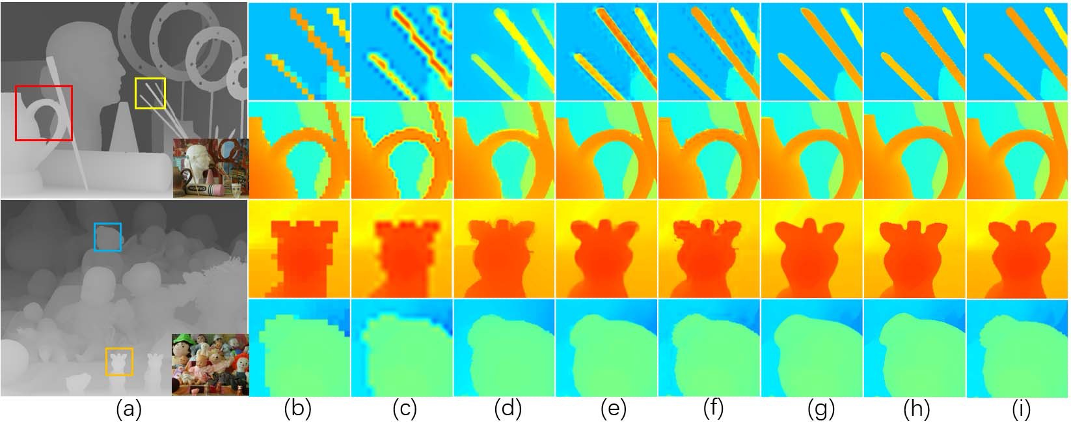
\includegraphics[width=.7\paperwidth]{figure/experiments1.png}
	\caption{在 Middlebury 数据集上不同模型在 $8\times$ 上采样结果的视觉比较。(a)真实深度图像和彩色图像;(b)低分辨率图像;(c)Bicubic;(d)JGF;(e)DGDIE;(f)DEIN;(g)GSRPT;(h)PMBANet;(i)真实深度图像。}
	\label{fig:experiment}
\end{figure*}

本文通过丰富的对比实验和消融实验验证了整体网络模型和所提出的创新性模块的有效性,其余实验不再赘述,以下为实验结果结论:

\begin{enumerate}
	\item[(1)] Middlebury Dataset (Noiseless Case): 为说明 PMBANet 的能力,将其与其他最新的深度图像超分辨率重建方法在不同的上采样倍率($4\times$,$8\times$ 和 $16\times$)进行比较。与基于 CNN 的方法相比(与基于 CNN 的方法相比,基于传统过滤或优化的方法可获得相对较高的 MAD 和 PE 值,即更差的性能),PMBANet 几乎获得了最佳的结果,尤其是在上采样倍率为 $8\times$ 和 $16\times$ 的情况下。在场景中较大的物体上,这些方法均取得了相似的结果,但只有 PMBANet 在微小的物体上仍能准确地恢复深度边界。
	\item[(2)] Middlebury Dataset (Noisy Case): GSRPT 和 PMBANet 可以在消除噪音的同时保持最清晰的深度边界。
	\item[(3)] 	NYU Datasset:在效率方面,PMBANet 在所有基于深度学习的方法中取得了最好的结果。
	\item[(4)] 	MPI dataset and Reak Data:在大部分情况下取得了优于其他方法的结果。
 
\end{enumerate}



%\begin{lstlisting}
%# \lstinputlisting{code/demo.py}
%import torch
%import torch.nn as nn
%
%print("pytorch")
%\end{lstlisting}

%\begin{algorithm}[H]
%        \caption{Joint Learning Strategy}
%        \LinesNumbered
%        \KwIn{Training data $D_{LR}$, $I_{HR}$, $D_{HR}$}
%        \KwOut{$D_{SR}$, $D_{DE}$}
%        Randomly initialize DSRNet and MDENet\\
%       
%        \For{ epoch=1; epoch $\leq$ 400;}
%        {
%         ——————————————— Step 1 ———————————————\\
%        $F_{MDE}=Encoder_{MDE}(I_{HR}^n)$\\
%        $F_{DSR}^{shallow}=Res^{(2)}(conv(D_{LR}))$ \tcp*{shallow feature extraction}
%        \For(\tcp*[f]{ i refers to $i^{th}$ layer of encoder}){i=1; i $\leq$ 3} 
%        {
%        \If{i=1}
%        {
%        $Fe_{DSR}^i=maxpool(Res^{(4)}(F_{DSR}^{shallow}))$\\
%        }
%        \Else{
%        $Fe_{DSR}^i=maxpool(Res^{(4)}(F_{ha}^{i-1}))$\\
%        }
%        $F_{blurred}^i=deconv(avgpool(F_{MDE}^i)$\\
%        $A_{hf}^i=PRelu(F_{MDE}^i-F_{blurred}^i)$\\
%        $F_{hg}^i=F_{MDE}^i+A_{hf}^i\cdot F_{MDE}^i$\\
%        $F_{comp}^i=[Fe_{DSR}^i,F_{hg}^i]$\\
%        $F_{ha}^i=SA(conv_{1\times 1}(CA(F_{comp}^i)))$\\
%        }
%        $F_{DSR}^{deeper}=Res^{(32)}(F_{ha}^3)$\\
%        $F_{DSR}^{multi-scale}=conv(conv(conv(Fe_{DSR}^{shallow}+Fe_{DSR}^1)+F_{DSR}^2)+Fe_{DSR}^3)$\tcp*{multi-scale features fusion}
%        $F_{DSR}^{fusion}=Res^{(2)}(F_{DSR}^{deeper}+F_{DSR}^{multi-scale})$\\
%        $F_{DSR}^{low-freq}=Downsample(F_{DSR}^{shallow})$\\
%        \For(\tcp*[f]{ j refers to $j^{th}$ layer of decoder}){i=1; i $\leq$ 3} 
%        {
%        \If{i=1}
%        {
%        $Fd_{DSR}^j=pixelshuffle(conv(F_{DSR}^{fusion}+F_{DSR}^{low-freq}))$\\
%        }
%        \Else{
%        $Fd_{DSR}^j=pixelshuffle(conv(F_{DSR}^{j-1}))$\\
%        }
%        }
%        $D_{SR}=conv_{1 \times 1}(Fd_{DSR}^3)$\\
%        Update weights of parts related to DSR with $\mathcal{L}_{DSR}=||D_{SR}-D_{HR}||_1$\\
%        ——————————————— Step 2 ———————————————\\
%        $F_{MDE}=Encoder_{MDE}(I_{HR}^n)$\\
%        \For{k=1;k $\leq$ 4}
%        {
%        \If{k=1}
%        {
%        $Fp_{MDE}^k=conv(Fe_{MDE}^{5-k})$
%        }
%        \Else
%        {
%        $Fe_{MDE}^{5-k}=interpolate(Fe_{MDE}^{5-k})$\\
%        $Fp_{MDE}^k= conv(Fe_{MDE}^{5-k} +Fe_{MDE}^{5-(k+1)})$
%        }
%        }   
%        \For{j=1;k $\leq$ 3}
%        {
%        \If{j=1}
%        {
%        $Fd_{MDE}^j=CLIFF(Fp_{MDE}^1,Fp_{MDE}^2)$\\
%        }
%        \Else
%        {
%        $M_{DSR}^j=conv_{1\times1}(Fd_{DSR}^j)$\\
%        $M_{MDE}^j=conv_{1\times1}(Fd_{MDE}^j)$\\
%        $W_{diff}^j=softmax(conv_{1\times1}(M_{DSR}^j-M_{MDE}^j))$\\
%        $F_{ca}^j=Fd_{DSR}^j+W_{diff}^j\ast Fd_{DSR}^j$\\
%        $F_{con}^j=[Fd_{MDE}^j,F_{ca}^j]$\\
%        $F_{cg}^j=SA(conv_{1\times1}(CA(F_{con}^j)))$\\
%        $Fd_{MDE}^j=CLIFF(F_{cg}^j,Fp_{MDE}^{j+1})$\\
%        }
%        }
%        $D_{DE}=interpolate(conv_{1\times 1}(Fd_{MDE}^3))$\\
%        Update weights of parts related to MDE with $\mathcal{L}_{MDE}=||D_{DE}-D_{HR}||_1$
%        }
%    \end{algorithm}

\end{document}
